\documentclass{article}

\usepackage{titlesec}
\usepackage{titling}
\usepackage[margin=0.7cm]{geometry}
\usepackage{float} 
\usepackage{graphicx}
\graphicspath{ {../img/} }
\usepackage{multirow}
\usepackage{booktabs}
\usepackage{hyperref}
\usepackage{xcolor}

\titleformat{\section}
{\Large\bfseries}
{}
{0em}
{}[\titlerule]

\titleformat{\subsection}
{\bfseries}
{}
{0em}
{}

\titleformat{\subsubsection}[runin]
{\bfseries}
{}
{0em}
{}

\titlespacing{\section}
{0em}{0em}{0.3em}
\titlespacing{\subsection}
{0em}{0em}{0em}
\titlespacing{\subsubsection}
{0em}{0em}{0.5em}

\setlength\intextsep{0mm}


\hypersetup{
  colorlinks=true,
  urlcolor=black!70!black
}

\begin{document}
\title{R\'esumm\'e}
\author{Carlos Herrera Valerio}



\begin{table}[ht]
\centering
	\begin{tabular}{p{5cm}p{6cm}p{6cm}}
	\multirow[t]{3}{*}[-2.3cm]{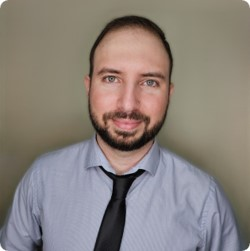
\includegraphics[width=0.16\textwidth]{profile_photo_1-1_rounded}} &
	\multicolumn{2}{c}{\huge\textbf{Carlos Herrera Valerio}} \\ &
	\begin{tabular}[c]{@{}l@{}}
		\\Electronic Engineer\\ 
		8+ years of experience\\ 
		Data Science\\ 
		Analog testing
	\end{tabular} &
		\multicolumn{1}{r}{
			\begin{tabular}[c]{@{}r@{}}
				\\(+506) 8894 4826\\ 
				\href{mailto:carlos.herrera.valerio@gmail.com}{carlos.herrera.valerio@gmail.com}\\ 
				\href{https://www.linkedin.com/in/carlosherreravalerio/}{linkedin.com/in/carlosherreravalerio}\\ 
				Heredia, Costa Rica
			\end{tabular}} \\
 &
\end{tabular}
\vspace{-12pt}
\end{table}

\section{About me}
\noindent
Experienced electronic engineer with over eight years in the semiconductor industry specializing in high-volume manufacturing, analog testing and electronic design validation of high speed IOs. Open to data science and data analytics career growth opportunities to align my job with my passion applying analysis to drive positive impact and innovation in the industry.

\section{Work Experience}
\subsection{Intel Costa Rica(2016 - Present day)}
\subsubsection{IO Design Validation of DDR Memory}
\subsubsection{2023 - Present day:}
Expanded expertise in utilizing laboratory equipment to characterize the analog capacity of DDR memory ports in Intel Xeon 6 products. Implemented automated data collection and analysis using a database and a GUI developed with JMP/JSL, reducing the time required to generate a single test report by 80\%.
\subsubsection{IO High Volume Manufacture}
\subsubsection{2022 - 2023:}
Collaborated remotely as module lead with the High-Speed IO team in the US on Intel’s 5th Gen Xeon project. Enabled full test content implementation within an aggressive schedule, frequently debugging Python scripts, actively participating in task force meetings with designers and validation teams to fine tune Gen5 test for UPI interfaces. As a result of this work, I was recognized for a remarkable, results-oriented effort.
\subsubsection{2019 - 2022:}
Led the team as Product Owner to fine tune PCIE health indicators, meeting quality goals through an analytical approach to early identify defects in the production line. Collaborated closely with designers and production teams to ensure product quality and achieve the DPM objective on schedule for the roadmap.
\subsubsection{2018:}
Successfully collaborated with a transnational team overseas to resolve a yield issue with Intel’s 10th Gen Client products. Contributed significantly through design of experiments (DoE), integration, data analysis, and data review. Successfully reduced DPM to meet the desired quality goal, gaining valuable experience in international collaboration and complex problem-solving with a diverse team.

\section{Skills}
\noindent\textbf{Data Analysis:} Analyze vast amounts of data to identify opportunities for production improvements, pulling information from databases to create informative charts to present and communicate insights to other engineering teams to define an action plan.\\
\textbf{Electronic Lab Equipment:} Use of lab equipment such as Scope, BERT, DCPA, VNA, switches, and thermal controllers. Automating tasks utilizing SCPI commands and python libraries.\\
\textbf{Programming:} Experienced in writing and reading code following professional standards to contribute in modular development. Enthusiastic about using Machine Learning methods to solve problems.\\
\textbf{Programming languages/libraries:} Proficient in Python, JMP/JSL, R, PySpark, Docker, PyTorch, Pandas, Matplotlib, Numpy, SeaBorn, Matplotlib, Sklearn, Postgres, SQL, Tableau.\\
\textbf{GNU/Linux:} Comfortable working within Linux dev-env running simulations, automating, managing files and using \LaTeX .\\
\textbf{Languages:} Excellent written and verbal communication skills in English, and native in Spanish.\\
\textbf{Team Work:} Actively participate in multidisciplinary engineering teams to address silicon issues, debug test content, reduce high fallout. Frequently analyze large volumes of data to select DUTs for specific DoEs, and communicate findings in sync meetings.\\
\textbf{Self-driven:} Constantly dealt with challenges and aggressive deadlines following Scrum methodology to divide a problem into multiple steps to ensure successful completion of a project.\\
\textbf{Problem-Solving:} Organized and strategic when facing a problem, finding underlying root cause, and focus on solutions, often implementing innovative alternatives. \\
\textbf{Result Oriented:} Always worked as a data driven and project oriented employee to deliver quality results. 

\section{Education}

\begin{table}[ht]
\centering
\begin{tabular}{lr}
	\begin{tabular}[c]{@{}l@{}}\textbf{FundaTec}\\ Data Science Program\end{tabular}                                                                                                                                                & \begin{tabular}[c]{@{}r@{}}\textbf{Cartago, Costa Rica}\\ Graduated September 2024\end{tabular}     \\
		\begin{tabular}[c]{@{}l@{}}\textbf{Costa Rica Institute of Tecnology(TEC)}\\ Licentiate Electronic Engineering\end{tabular}                                                                                                     & \begin{tabular}[c]{@{}r@{}}\textbf{Cartago, Costa Rica}\\ Graduated June 2016\end{tabular}     \\
			\begin{tabular}[c]{@{}l@{}}\textbf{University Center Miravalles}\\ Professional Development Program (PDP)\\ Reinforcement of soft skills, integrity, communication, emotional intelligence and abilities for life.\end{tabular} & \begin{tabular}[c]{@{}r@{}}\textbf{San Jose, Costa Rica}\\ Graduated December 2015\end{tabular}
\end{tabular}
\end{table}

\section{References}
\begin{flushleft}
	Didier Chacón | Manager from 2019 to 2023: \href{mailto:didier.o.chacon.barquero@intel.com}{didier.o.chacon.barquero@intel.com} | (+506) 2298 7940 \\
	Timothy Jones | US High-Speed IO Manager: \href{mailto:timothy.l.jones@intel.com}{timothy.l.jones@intel.com} | +1 (408) 765-5694 \\
	Enrique Con | Product Owner and peer: \href{mailto:enriqueconh@yahoo.com}{enriqueconh@yahoo.com} | (+506) 8866 4820 \\

%Gustavo Aguilar | Mentor \\

\end{flushleft}

\end{document}
